\chapter{Results and Analysis} \label{Chap4}
\section{Configurations} % done chat, turnitin
The evaluation is configured as follows:
\begin{enumerate}[nolistsep]
    \item Metrics: The evaluation focuses on two main metrics, the total number of additional swap gates $(g)$ and the resulting circuit depth $(d)$ after transpilation.
    \item Experiment Software: The algorithm is implemented in Python version 3.10.12 with IBM Qiskit framework. The code is available on Github \url{https://github.com/natashaval/qubit-mapping-distributed-qc}.
    \item Experiment Hardware: The tests were conducted on a standard personal computer equipped with an Intel i7-8700 CPU and 16 GB of RAM.
    \item Layout: The algorithms were tested using 20 qubits across the layouts detailed in Table  \ref{tab:layout-qubit-group}. The layout names follow the format: \textit{<layout name>\_<number of qubits>\_<number of groups>}. Each layout is a symmetric coupling graph, enabling bidirectional operation of two-qubit gates between any pair of connected physical qubits. Coupling graphs are illustrated in Appendix \ref{app:dj-10-layout}.
        \begin{table}[htb]
\centering
\caption{Number of qubits and group for layouts}
\label{tab:layout-qubit-group}
\begin{tabular}{|c|c|c|} 
\hline
\textbf{Layout} & \textbf{Number of qubits} & \textbf{Number of groups}  \\ 
\hline
Full            & 20                        & 1                         \\ 
\hline
Full            & 10                        & 2                         \\ 
\hline
Grid            & 9                         & 2                         \\ 
\hline
Ring            & 10                        & 2                         \\ 
\hline
Full            & 7                         & 3                         \\ 
\hline
Grid            & 8                         & 3                         \\ 
\hline
Ring            & 7                         & 3                         \\ 
\hline
Full            & 5                         & 4                         \\ 
\hline
Grid            & 6                         & 4                         \\ 
\hline
Ring            & 5                         & 4                         \\ 
\hline
T Horizontal    & 5                         & 4                         \\ 
\hline
T Vertical      & 5                         & 4                         \\ 
\hline
Line            & 1                         & 20                        \\
\hline
\end{tabular}
\end{table}
    \item Benchmarks: The benchmarks  listed in Table \ref{tab:table-algorithm-size-depth} are taken from MQTBench \cite{quetschlich_mqt_2023}. The quantum circuits are composed of native gates from the Qiskit library and are represented in the QASM 2.0 language.
        \begin{table}[htb]
\centering
\caption{Circuit size and circuit depth of benchmark algorithms for 5, 10, and 15 qubits}
\label{tab:table-algorithm-size-depth}
\begin{tabular}{|l|c|c|c|c|c|c|} 
\hline
\multicolumn{1}{|c|}{\textbf{Algorithm}} & \multicolumn{2}{c|}{\textbf{n = 5}} & \multicolumn{2}{c|}{\textbf{n = 10}} & \multicolumn{2}{c|}{\textbf{n = 15}}  \\ 
\hline
\multicolumn{1}{|c|}{\textbf{}}          & gate & depth                        & gate & depth                         & gate & depth                          \\ 
\hline
ghz                                      & 7    & 7                            & 12   & 12                            & 17   & 17                             \\ 
\hline
dj                                       & 36   & 11                           & 79   & 17                            & 118  & 22                             \\ 
\hline
graphstate                               & 50   & 22                           & 100  & 26                            & 150  & 29                             \\ 
\hline
qft                                      & 71   & 38                           & 270  & 78                            & 591  & 118                            \\ 
\hline
wstate                                   & 73   & 45                           & 163  & 90                            & 253  & 135                            \\ 
\hline
qftentangled                             & 78   & 42                           & 282  & 82                            & 608  & 122                            \\ 
\hline
vqe                                      & 83   & 21                           & 168  & 26                            & 253  & 31                             \\ 
\hline
qaoa                                     & 95   & 31                           & 190  & 34                            & 285  & 34                             \\ 
\hline
realamprandom                            & 130  & 37                           & 335  & 57                            & 615  & 77                             \\ 
\hline
twolocalrandom                           & 130  & 37                           & 335  & 57                            & 615  & 77                             \\ 
\hline
su2random                                & 150  & 41                           & 375  & 61                            & 675  & 81                             \\ 
\hline
qnn                                      & 154  & 58                           & 459  & 108                           & 914  & 158                            \\ 
\hline
portfolioqaoa                            & 195  & 72                           & 615  & 132                           & 1260 & 192                            \\ 
\hline
random                                   & 223  & 97                           & 646  & 155                           & 1992 & 412                            \\ 
\hline
portfoliovqe                             & 310  & 107                          & 1145 & 217                           & 2505 & 327                            \\
\hline
\end{tabular}
\end{table}
\end{enumerate}

\section{Evaluation}
The data is processed from the table in the appendix \ref{app:benchmark-result-table-by-group}.
\subsection{Distribution of Additional Swap Gates and Circuit Depth} % done chat
The box plot in Figure \ref{fig:chart-box-plot-swap} compares the average number of additional swap gates required by three different strategies, namely \lstinline{BasicSwap}, \lstinline{SabreSwap}, and \lstinline{LookaheadSwap}, across various layout configurations. \lstinline{BasicSwap} \cite{ibmquantum_basicswap} strategy employs a brute force approach, adding one or more swap gates whenever a connectivity constraint is encountered, iterating through each layer until the circuit is compatible. The \lstinline{SabreSwap} strategy uses a heuristic search to minimize the number of swap gates and reduce circuit depth \cite{li_tackling_2019, ibmquantum_sabreswap}. Meanwhile, the \lstinline{LookaheadSwap} strategy combines elements from both algorithms (Algorithm \ref{alg:interaction-layout-mapping} and \ref{alg:lookahead-swap-routing}) that has been described in the previous section. A lower number of swap gates or fewer circuit depth indicates better strategy performance. \\
The \lstinline{BasicSwap} consistently exhibits the highest number of swap gates across all layouts, with particularly high values exceeding 5000 additional swap gates in layouts such as \textit{ring\_10\_2}, \textit{t\_horizontal\_5\_4}, \textit{t\_vertical\_5\_4}, and performing worst in the \textit{line\_1\_20} layout. The large spread and height of the boxes indicate both poor and inconsistent performance. In contrast, \lstinline{SabreSwap} performs significantly better with the range of around 1000 additional swap gates for all layouts. \lstinline{LookaheadSwap} performs almost as well as \lstinline{SabreSwap}, with the best results seen in the \textit{full\_7\_3} layout. However, in some cases like \textit{full\_5\_4} and \textit{ring\_5\_4}, the \lstinline{LookaheadSwap} strategy has exceptionally low values that are likely outliers due to timeouts, which may skew the perception of its effectiveness in these instances. \\
Overall, the layouts that show better performance, as indicated by lower swap gate counts, are \textit{grid\_8\_3}, \textit{grid\_6\_4}, \textit{full\_10\_2} and \textit{full\_7\_3}. These results suggest that \textit{grid} and \textit{full} layouts are generally more efficient than other configurations. It is also important to note that \textit{full\_20\_1} and \textit{line\_1\_20} serve as baselines; \textit{full\_20\_1} represents a maximally connected coupling map and is expected to deliver the best performance, while \textit{line\_1\_20}, being the least connected, is likely to show the poorest performance. \\
\begin{figure}[htb]
    \centering
    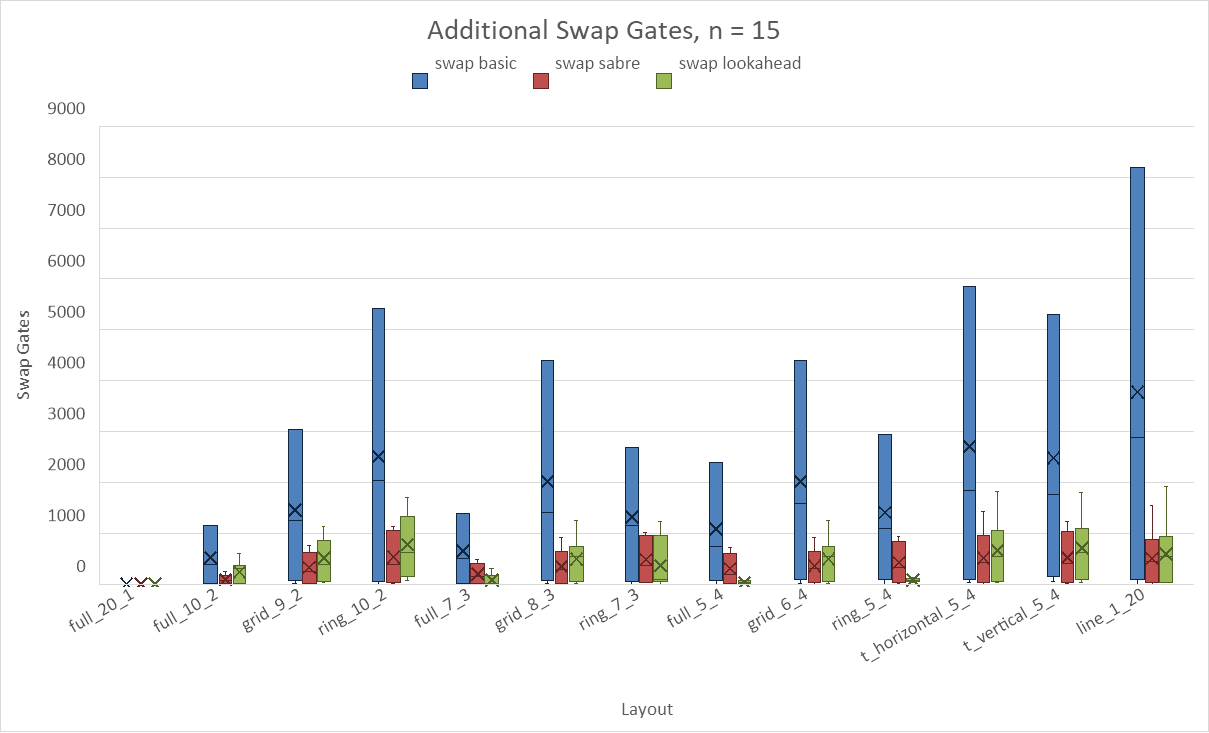
\includegraphics[width=0.9\linewidth]{image/chart_box_plot_swap.png}
    \caption{Box plot additional swap gates for a circuit size of 15}
    \label{fig:chart-box-plot-swap}
\end{figure}

Similarly, the analysis of quantum circuit depths across various layouts, as shown in Figure \ref{fig:chart-box-plot-depth}, reveals significant differences in the effectiveness of the three optimization methods. The depths associated with \lstinline{BasicSwap} consistently result in the highest circuit depths often exceeding 1000, and in some cases approach 2000 or more in layouts like \textit{line\_1\_20}, \textit{t\_horizontal\_5\_4}, and \textit{ring\_10\_2}. In contrast, \lstinline{SabreSwap} and \lstinline{LookaheadSwap} both achieve significantly shallower circuit depths, generally clustering below 500. However, some layouts, such as \textit{full\_5\_4} and \textit{ring\_5\_4} show occasional outliers. \\
Overall, the \lstinline{SabreSwap} and \lstinline{LookaheadSwap} strategies perform comparably well, with the latter slightly outperforming \lstinline{SabreSwap} in certain configurations. The most efficient layouts, characterized by lower circuit depths, include \textit{full\_7\_3} and \textit{grid\_6\_4}, where both \lstinline{SabreSwap} and \lstinline{LookaheadSwap} consistently maintain minimal circuit depth. This suggests that for minimizing circuit depth, \lstinline{LookaheadSwap} is generally the most effective strategy, closely followed by \lstinline{SabreSwap}.
\begin{figure}[htb]
    \centering
    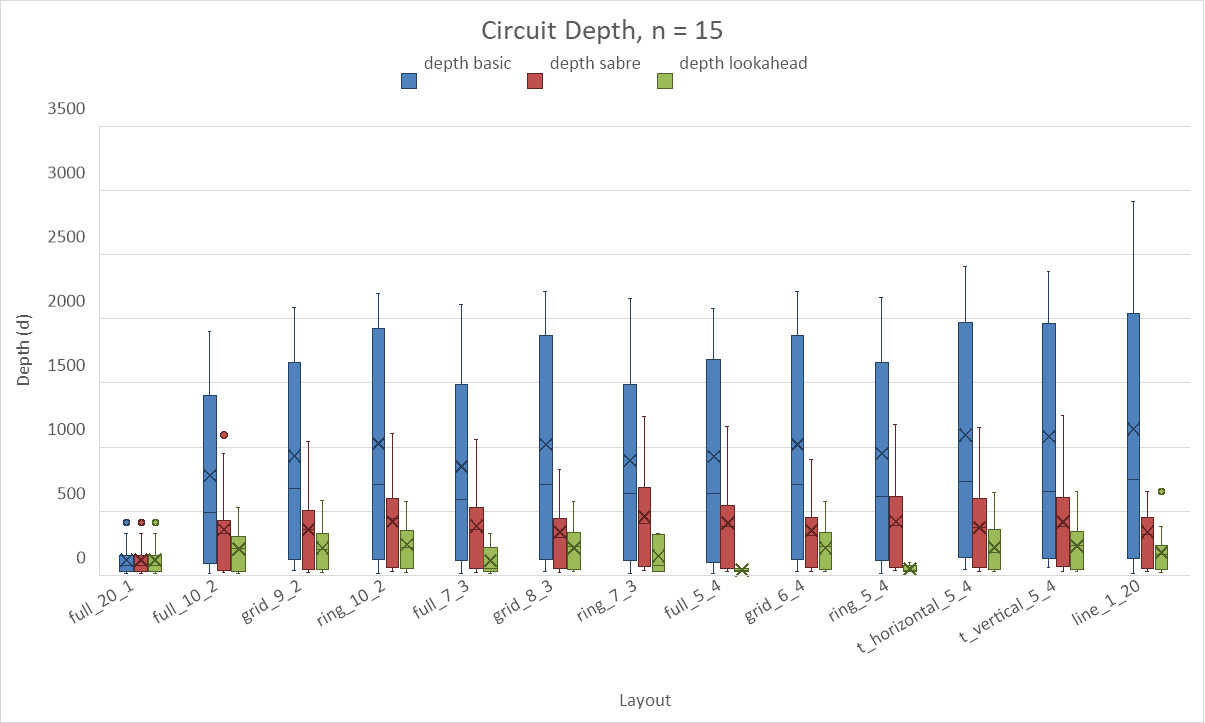
\includegraphics[width=\linewidth]{image/chart_box_plot_depth.png}
    \caption{Box plot circuit depth for a circuit size of 15}
    \label{fig:chart-box-plot-depth}
\end{figure}

The box plots present the additional swap gates \ref{fig:chart-box-plot-group} and circuit depth \ref{fig:chart-box-plot-group-depth} categorized by group for a circuit size of 15.  Group 1 and Group 20 serve as baselines, with Group 1 representing a fully connected graph and Group 20 a line coupling graph. Among other groups, Group 2 stands out as the best performer. In Group 2, the \lstinline{LookaheadSwap} strategy performs particularly well, showing very low swap gate counts and moderate circuit depths, reflecting consistent and efficient performance. Group 3, while similar to Group 2, displays slightly more variability in circuit depths and a minor increase in swap gate counts, particularly with the \lstinline{BasicSwap} strategy, though the \lstinline{LookaheadSwap} approach still outperforms the others. Group 4, on the other hand, shows the most variability, especially with the \lstinline{BasicSwap} strategy, which has a much higher median and a widespread, suggesting inconsistent performance. Although the \lstinline{LookaheadSwap} strategy in Group 4 still achieves the lowest swap gate counts and circuit depths, its performance is less consistent compared to Groups 2 and 3. Therefore, Group 2 emerges as the top performer in minimizing swap gates and lowering circuit depths with the \lstinline{LookaheadSwap} strategy, followed by Group 3, while Group 4 shows the least favourable results. \\
\begin{figure}[htb]
    \centering
    \begin{subfigure}{0.48\linewidth}
        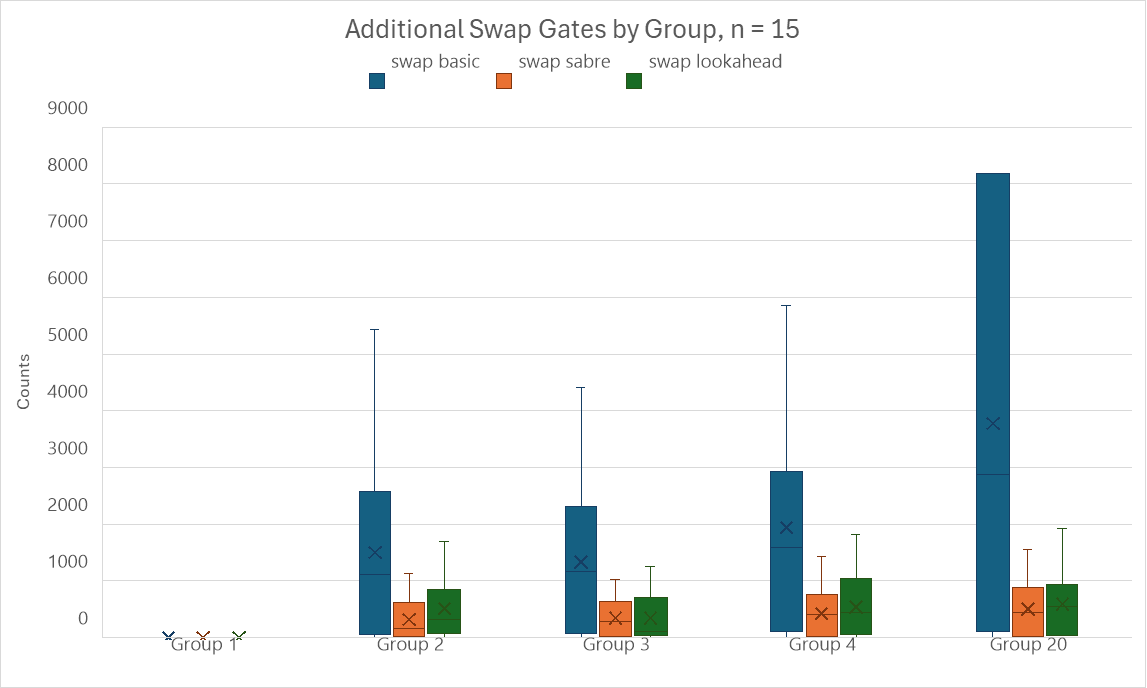
\includegraphics[width=\linewidth]{image/chart_box_plot_group.png}
        \caption{Box Plot Additional Swap Gates by Group}
        \label{fig:chart-box-plot-group}
    \end{subfigure}
    \begin{subfigure}{0.48\linewidth}
        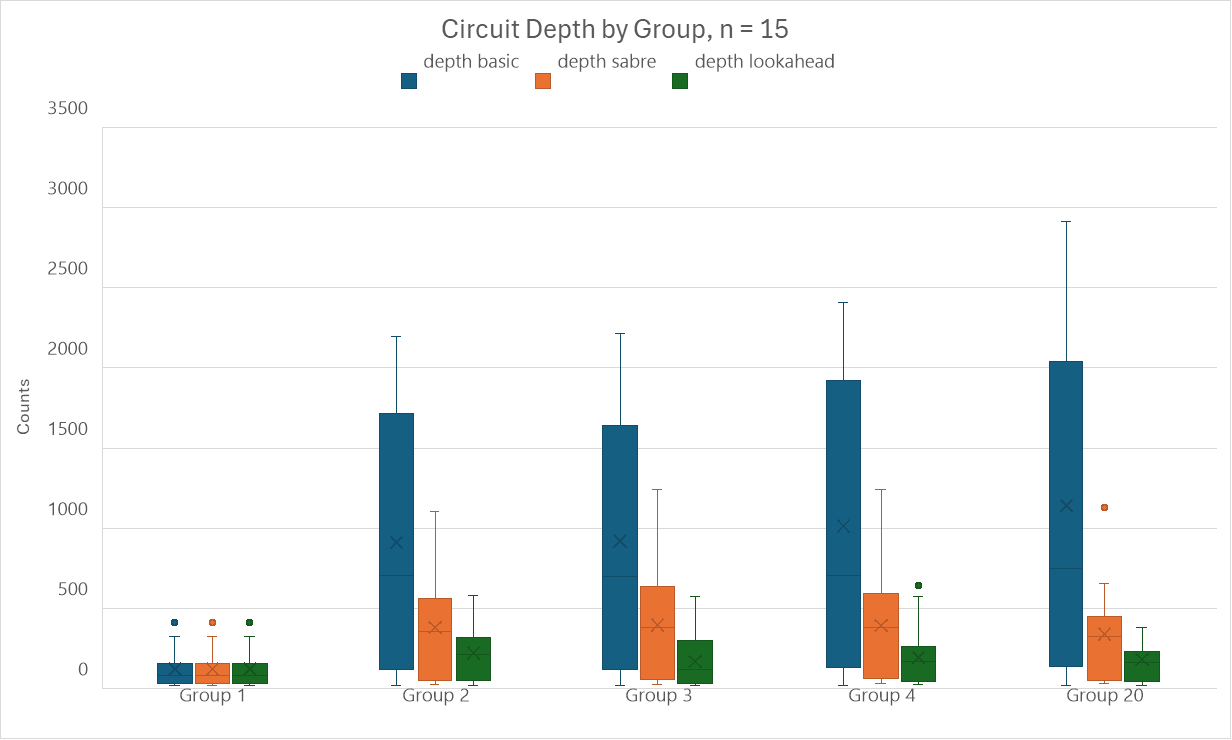
\includegraphics[width=\linewidth]{image/chart_box_plot_group_depth.png}
        \caption{Box Plot Circuit Depth by Group}
        \label{fig:chart-box-plot-group-depth}
    \end{subfigure}
    \caption{Swap strategies categorized in group for a circuit size of 15}
    \label{fig:chart-box-plot-group-all}
\end{figure}

\subsection{The Total Number of Algorithms Successfully Run for Each Layout}
The previous section mentioned that the algorithms for the \textit{full\_5\_4} and \textit{ring\_5\_4} layouts show outliers, indicating that they do not execute all the algorithms. Therefore, the chart in Figure \ref{fig:chart-success-algorithm-run} specifies the total number of successful algorithms run across different layouts, focusing on circuit sizes ranging from 5, 10, and 15 qubits, with a total of 15 algorithms per round. Most layouts perform consistently well, achieving the maximum count of 15 successful runs per benchmark. \\
One thing to notice is that \textit{full\_7\_3} and \textit{full\_5\_4}  layouts fail to complete the benchmarks for the largest circuit size of 15 qubits, with \textit{full\_7\_3} achieving only 9 successful runs and \textit{full\_5\_4} barely completing 3 runs. Additionally, \textit{ring\_7\_3} and \textit{ring\_5\_4} layouts also encounter difficulties, particularly as the circuit size increases beyond 10 qubits. \textit{Ring\_7\_3} can only achieve 10 and 8 successful runs for circuit sizes 10 and 15, while \textit{ring\_5\_4} struggles even at the 5-qubit benchmark, with its performance worsening as the circuit size increases. The failed algorithms and layouts are listed in Appendix \ref{app:failed-algorithm-layout}. \\
These variations suggest that certain layouts are more robust across different run sizes, while others, particularly \textit{ring\_7\_3} and \textit{ring\_5\_4} face challenges with medium run sizes, indicating possible inefficiencies or challenges in these configurations. In general, the layouts in groups 1 and 2 are more consistent across different run sizes, while those in groups 3 and 4 tend to show more variability.
\begin{figure}[htb]
    \centering
    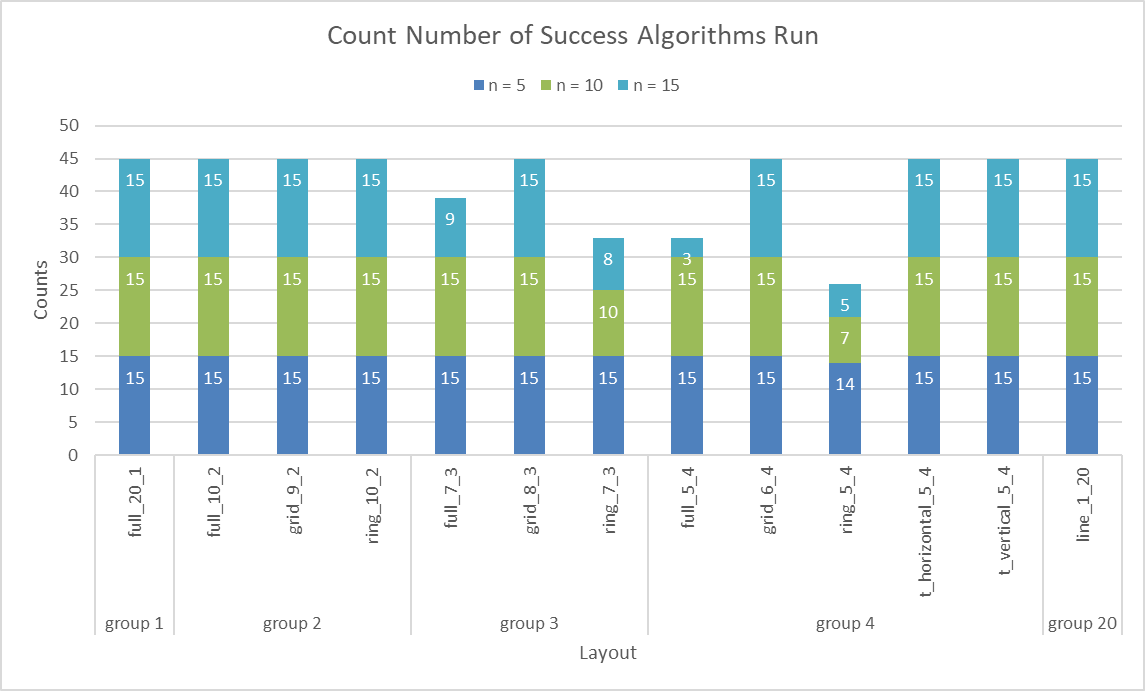
\includegraphics[width=0.8\linewidth]{image/chart_success_algorithm_run.png}
    \caption{Total count of successful algorithm runs across various layouts, $n = 15$}
    \label{fig:chart-success-algorithm-run}
\end{figure}

In addition, the chart in Figure \ref{fig:chart-success-layout-run} highlights the total count of successful layout executions across different algorithms. Most algorithms like "dj", "graphstate" and "qaoa" maintain consistent performance across all benchmark sizes with 100\% success rate. However, some algorithms, like "qft", "qftentangled", "realamprandom", and "twolocalrandom", show slightly reduced success rates, particularly for $n = 10$, where the count drops to 12. The algorithms "qnn" and "random" display even more pronounced variations, with success rates for $n = 10$ and $n = 15$ decreasing to 11 and 9, respectively. \\
While most algorithms perform reliably across all benchmarks, a few show inconsistencies, especially with $n = 10$ and $n = 15$, suggesting that certain algorithms may struggle with larger problem sizes.
\begin{figure}[htb]
    \centering
    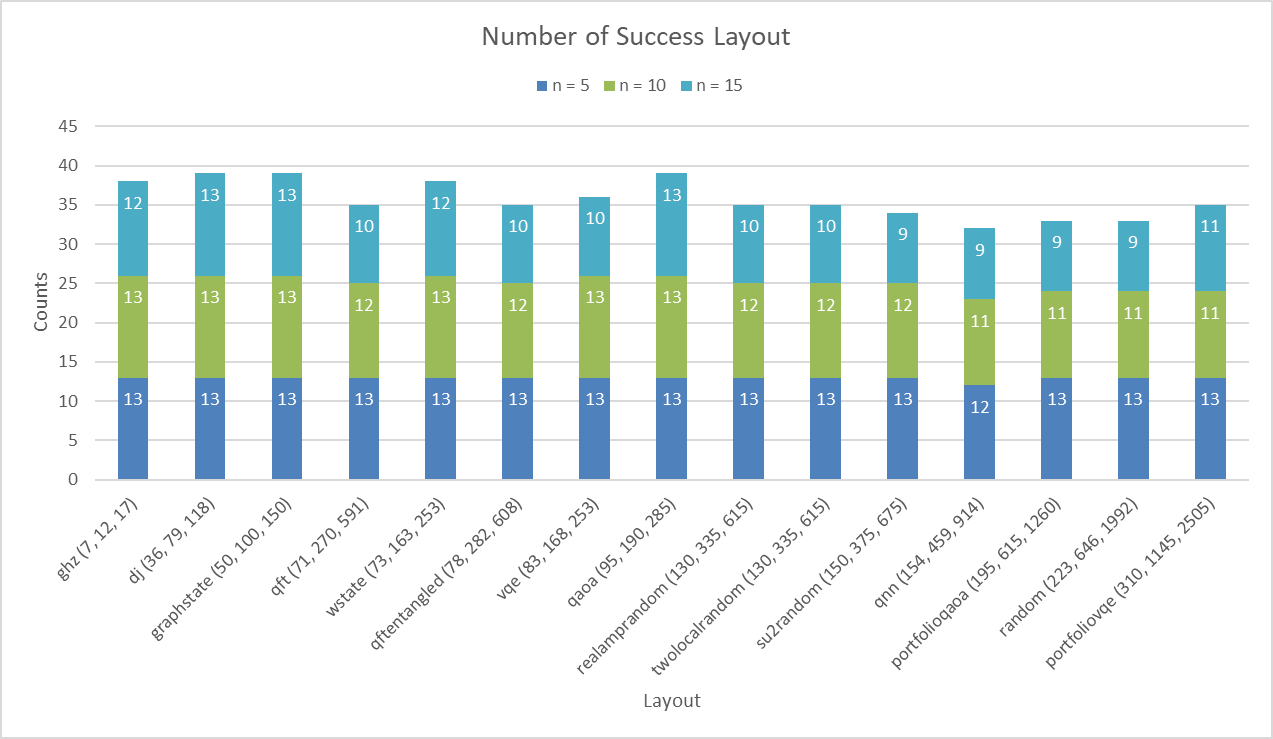
\includegraphics[width=0.8\linewidth]{image/chart_success_layout_run.png}
    \caption{Total count of successful layouts across different algorithms}
    \label{fig:chart-success-layout-run}
\end{figure}
\FloatBarrier

\subsection{Layouts for Algorithms}
In this section, a selection of representative algorithms - GHZ, Deutsch-Jozsa, Graph State, VQE, and Portfolio QAOA - are analyzed and compared across various layouts. The baseline values for the total circuit gates and circuit depth are provided in parentheses, and the results discussed are based on using 15 qubits. This comparison highlights how different layouts perform when subjected to different swap routing methods.

\subsection{GHZ} % done chat
The GHZ charts compare the number of additional swap gates needed for different layouts (Figure \ref{fig:chart-ghz}) and the resulting circuit depth (Figure \ref{fig:chart-ghz-depth}) when running with 17 qubits. It shows that the \lstinline{BasicSwap} strategy generally performs best, requiring the fewest swaps, particularly in all full, ring, and line layouts, where it results in 0 additional swap gates. In this context, \lstinline{SabreSwap} tend to perform worse than \lstinline{BasicSwap}, while the \lstinline{LookaheadSwap} strategy performs significantly worse than the others, with a notable spike in the \textit{ring\_10\_2} layout. Regarding circuit depth, the results for \lstinline{LookaheadSwap} are nearly comparable to those of \lstinline{SabreSwap}, with both strategies yielding a circuit depth of approximately 30.
\begin{figure}[htb]
    \centering
    \begin{subfigure}{0.48\linewidth}
        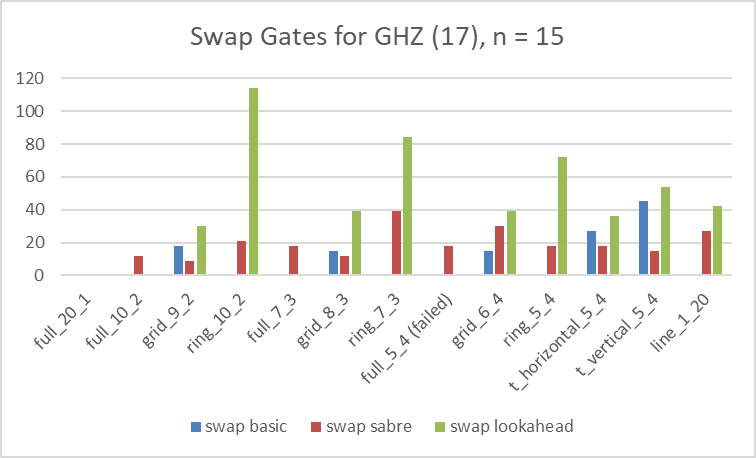
\includegraphics[width=\linewidth]{image/chart_ghz.png}
        \caption{Additional swap gates for GHZ}
        \label{fig:chart-ghz}
    \end{subfigure}
    \begin{subfigure}{0.48\linewidth}
        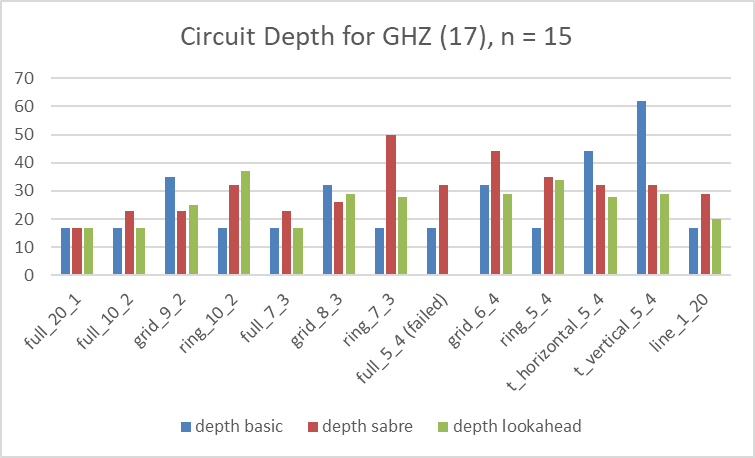
\includegraphics[width=\linewidth]{image/chart_ghz_depth.png}
        \caption{Circuit depth for GHZ}
        \label{fig:chart-ghz-depth}
    \end{subfigure}
\end{figure}

\subsection{Deutsch-Jozsa} % done chat
The charts for running the Deutsch-Jozsa algorithm with 118 gates (Figure \ref{fig:chart-dj}) and a circuit depth of 22 (Figure \ref{fig:chart-dj-depth}) show that the \lstinline{SabreSwap} and \lstinline{LookaheadSwap} strategies consistently outperform the \lstinline{BasicSwap} strategy in minimizing swap gates. The \textit{line\_20\_1} layout performs poorly, with the \lstinline{BasicSwap} method leading to an extremely high number of additional swap gates, exceeding 500. Although the additional swap gates for \lstinline{SabreSwap} and \lstinline{LookaheadSwap} are similar across all layouts, remaining below 50, the circuit depth with \lstinline{LookaheadSwap} is significantly lower, staying under 40 for all layouts, compared to \lstinline{SabreSwap}, which is around 60.
\begin{figure}[htb]
    \centering
    \begin{subfigure}{0.48\linewidth}
        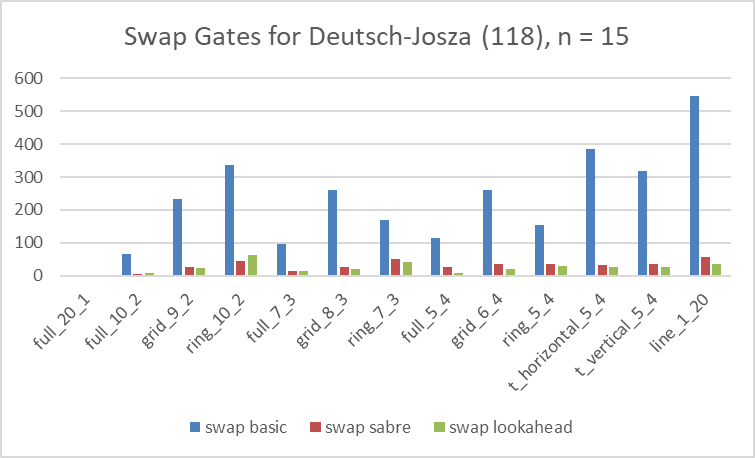
\includegraphics[width=\linewidth]{image/chart_dj.png}
        \caption{Additional swap gates for Deutsch-Jozsa}
        \label{fig:chart-dj}
    \end{subfigure}
    \begin{subfigure}{0.48\linewidth}
        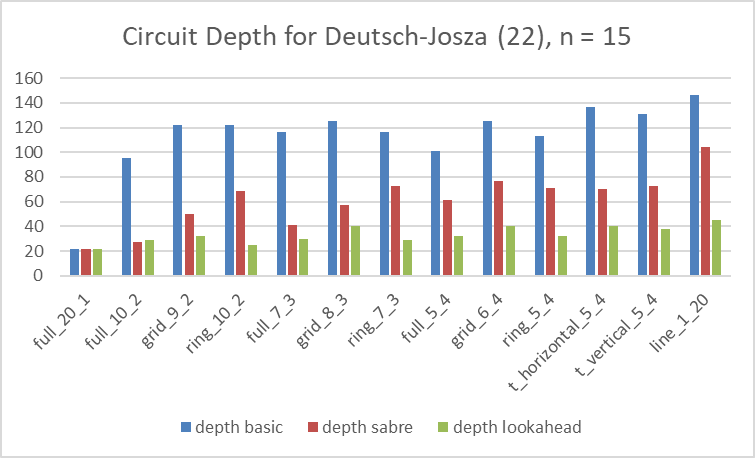
\includegraphics[width=\linewidth]{image/chart_dj_depth.png}
        \caption{Circuit depth for Deutsch-Jozsa}
        \label{fig:chart-dj-depth}
    \end{subfigure}
\end{figure}

\subsection{Graph State} % done chat
The Graph State charts compare additional swap gates with an initial count of 150 gates (Figure \ref{fig:chart-graphstate}) and a circuit depth of 30 (Figure \ref{fig:chart-graphstate-depth}) across different layouts. In this algorithm, the performance of \lstinline{LookaheadSwap} is similar to \lstinline{BasicSwap}, with the poorest performance observed in the \textit{t\_vertical\_5\_4} layout, which requires 120 additional swap gates. The \lstinline{SabreSwap} strategy, on the other hand, results in significantly fewer swap gates, with counts around 20. Despite the difference in additional swap gates between \lstinline{SabreSwap} and \lstinline{LookaheadSwap} being as much as 200\%, the resulting circuit depth is almost comparable, ranging from 30 to 40 across all layouts.
\begin{figure}[htb]
    \centering
    \begin{subfigure}{0.48\linewidth}
        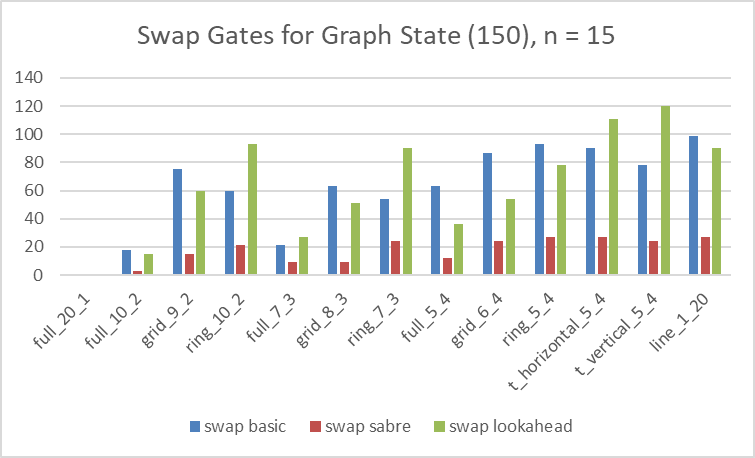
\includegraphics[width=\linewidth]{image/chart_graphstate.png}
        \caption{Additional swap gates for Graph State}
        \label{fig:chart-graphstate}
    \end{subfigure}
    \begin{subfigure}{0.48\linewidth}
        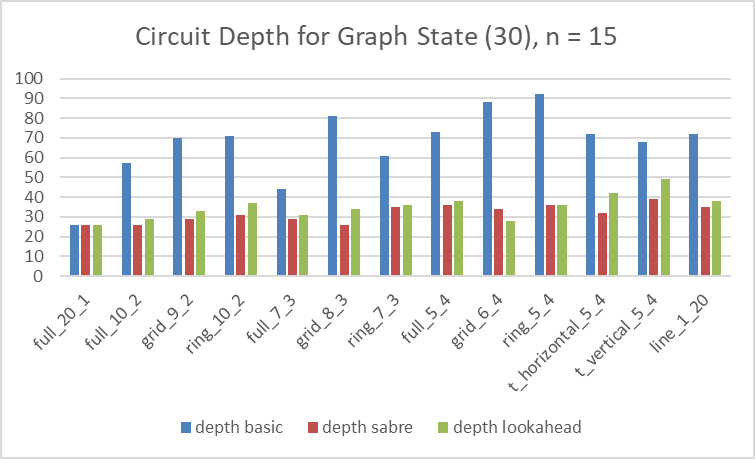
\includegraphics[width=\linewidth]{image/chart_graphstate_depth.png}
        \caption{Circuit depth for Graph State}
        \label{fig:chart-graphstate-depth}
    \end{subfigure}
\end{figure}

\subsection{VQE}
The chart illustrates that for the VQE algorithm with 253 gates (Figure \ref{fig:chart-vqe}), the \lstinline{SabreSwap} strategy generally performs best across most layouts, particularly in \textit{grid\_8\_3}, \textit{grid\_6\_4} and \textit{t\_horizontal\_5\_4}, where it minimizes the number of additional swap gates. In contrast, the \lstinline{LookaheadSwap} strategy tends to require significantly more swaps, especially in layouts like \textit{ring\_10\_2} and \textit{t\_vertical\_5\_4}. The \lstinline{BasicSwap} strategy shows similar behaviour to \lstinline{LookaheadSwap}, with the exception of the \textit{t\_vertical\_5\_4} layout, where it exceeds 140 additional swap gates. When examining circuit depth (Figure \ref{fig:chart-vqe-depth}), \lstinline{BasicSwap} does not show much difference from the baseline, remaining at 31. Meanwhile, the circuit depth performance of \lstinline{LookaheadSwap} is comparable to that of \lstinline{SabreSwap}, with layouts like \textit{full\_7\_3} and \textit{t\_vertical\_5\_4} delivering significantly better results, with a reduction of nearly 40\%.
\begin{figure}[htb]
    \centering
    \begin{subfigure}{0.48\linewidth}
        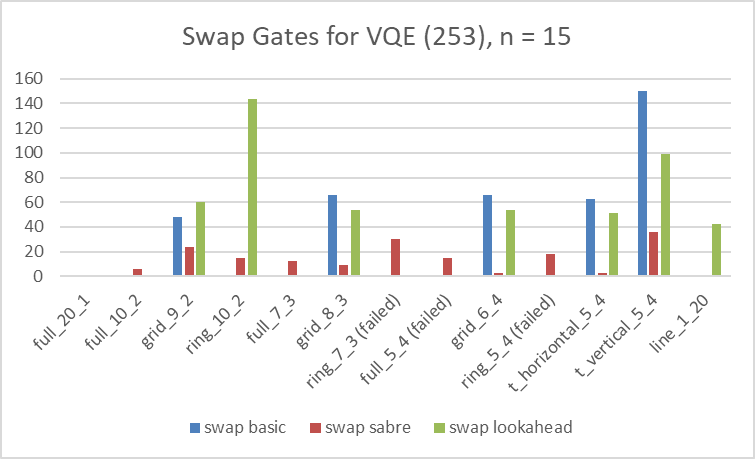
\includegraphics[width=\linewidth]{image/chart_vqe.png}
        \caption{Additional swap gates for VQE}
        \label{fig:chart-vqe}
    \end{subfigure}
    \begin{subfigure}{0.48\linewidth}
        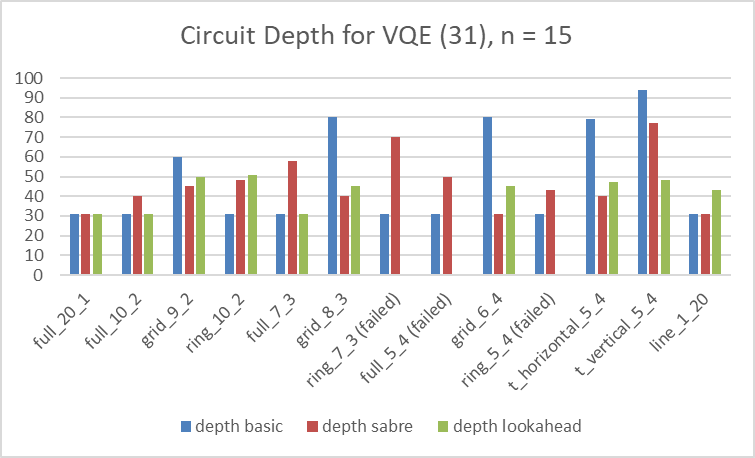
\includegraphics[width=\linewidth]{image/chart_vqe_depth.png}
        \caption{Circuit depth for VQE}
        \label{fig:chart-vqe-depth}
    \end{subfigure}
\end{figure}

\subsection{Portfolio QAOA}
These final charts serve as representatives for various other algorithms listed in Table \ref{tab:table-algorithm-size-depth}, ranging from "qft" to "portfoliovqe". The charts compare the performance of swap strategies for the Portfolio QAOA algorithm with 1260 gates (Figure \ref{fig:chart-portfolioqaoa}) and a circuit depth of 192 (Figure \ref{fig:chart-portfolioqaoa-depth}). The \lstinline{BasicSwap} strategy performs poorly, especially in layouts like \textit{ring\_10\_2}, \textit{t\_horizontal\_5\_4}, and \textit{line\_1\_20} with swap counts exceeding 5000 in some cases. On the other hand, both \lstinline{SabreSwap} and \lstinline{LookaheadSwap} significantly reduce the number of swap gates across most layouts to just below 2000, with \lstinline{SabreSwap} generally requiring fewer swaps than \lstinline{LookaheadSwap}. The second chart showing circuit depth follows a similar pattern: \lstinline{BasicSwap} results in much deeper circuits, often exceeding 2000 in depth, particularly in the same problematic layouts. \lstinline{SabreSwap} and \lstinline{LookaheadSwap} again perform better, with \lstinline{SabreSwap} consistently achieving lower circuit depths around 700, closely followed by \lstinline{LookaheadSwap} just below 500.
\begin{figure}[htb]
    \centering
    \begin{subfigure}{0.48\linewidth}
        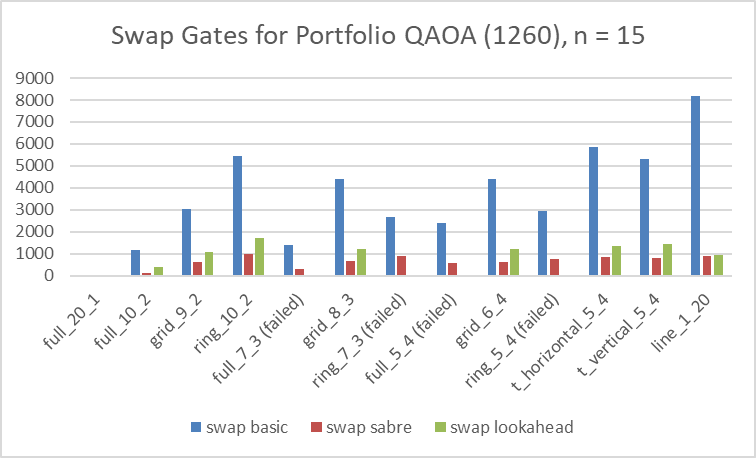
\includegraphics[width=\linewidth]{image/chart_portfolioqaoa.png}
        \caption{Additional swap gates for Portfolio QAOA}
        \label{fig:chart-portfolioqaoa}
    \end{subfigure}
    \begin{subfigure}{0.48\linewidth}
        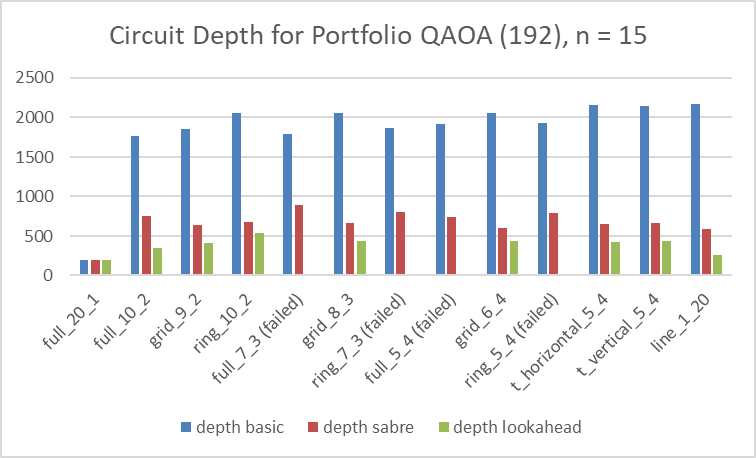
\includegraphics[width=\linewidth]{image/chart_portfolioqaoa_depth.png}
        \caption{Circuit depth for Portfolio QAOA}
        \label{fig:chart-portfolioqaoa-depth}
    \end{subfigure}
\end{figure}